\chapter{Introduction}
\label{ch1}

%%%%% https://cerncourier.com/a/pushing-the-precision-frontier/
% https://home.cern/news/news/physics/why-precision-luminosity-measurements-matter


\section{Particle Physics and the Standard Model}

Elementary particle physics is the study of the particles at the most fundamental level, the constituents of the universe as well as the interactions between them which are called, electromagnetic force, nuclear weak force and nuclear strong force and there is also the gravity force but this one doesn't have a satisfactory quantum theory for it. Each of these forces are mediated by exchange particles, in the case of the electromagnetic force the mediator is the photon, for the strong force the gluons, for the weak force the bosons W and Z and for the gravity we have the hypothetical graviton.  \cite{Griff}  

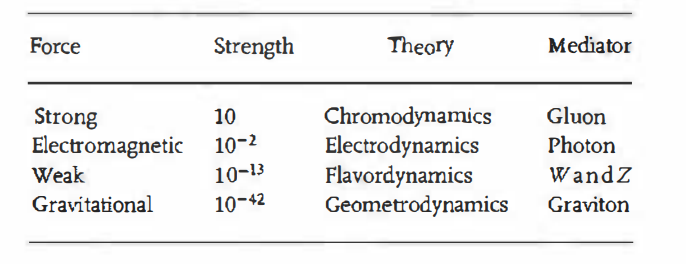
\includegraphics[scale=1]{table1.png}
\caption{Forces magnitude compared}

Each of these forces have a mathematical description for the physical systems of these interactions using the Quantum Field Theory (QFT). The one that describes systems under the electromagnetic force is called Quantum Electrodynamics (QED) this force dictates the electronic structure of atoms being the low energy manifestation of the electromagnetic theory. For the strong force Quantum Chromodynamics (QCD) is the fundamental theory of strong interactions, this force is responsible of maintaining protons and neutrons together in the atomic nucleus. For the weak interactions there is no particular name in the same way as the previous two, this force is is carried by all quarks and leptons and is responsible for the $\beta$ Decay of some radioactive isotopes and nuclear processes of the sun. \cite{mppthomson}   


Almost all the physical phenomena can be explained with only the electron, the electron neutrino, the proton and the neutron interacting with the electromagnetic force, the strong force and the weak one. When higher levels of energy are present new particles are observed, all of this is known as the elementary particles which are embodied in the standard model of particle physics that is by far the best theorical model that describes interaction of this elementary particles. Is divided into two categories the bosonic sector and the fermionic sector.  \cite{mppthomson}   

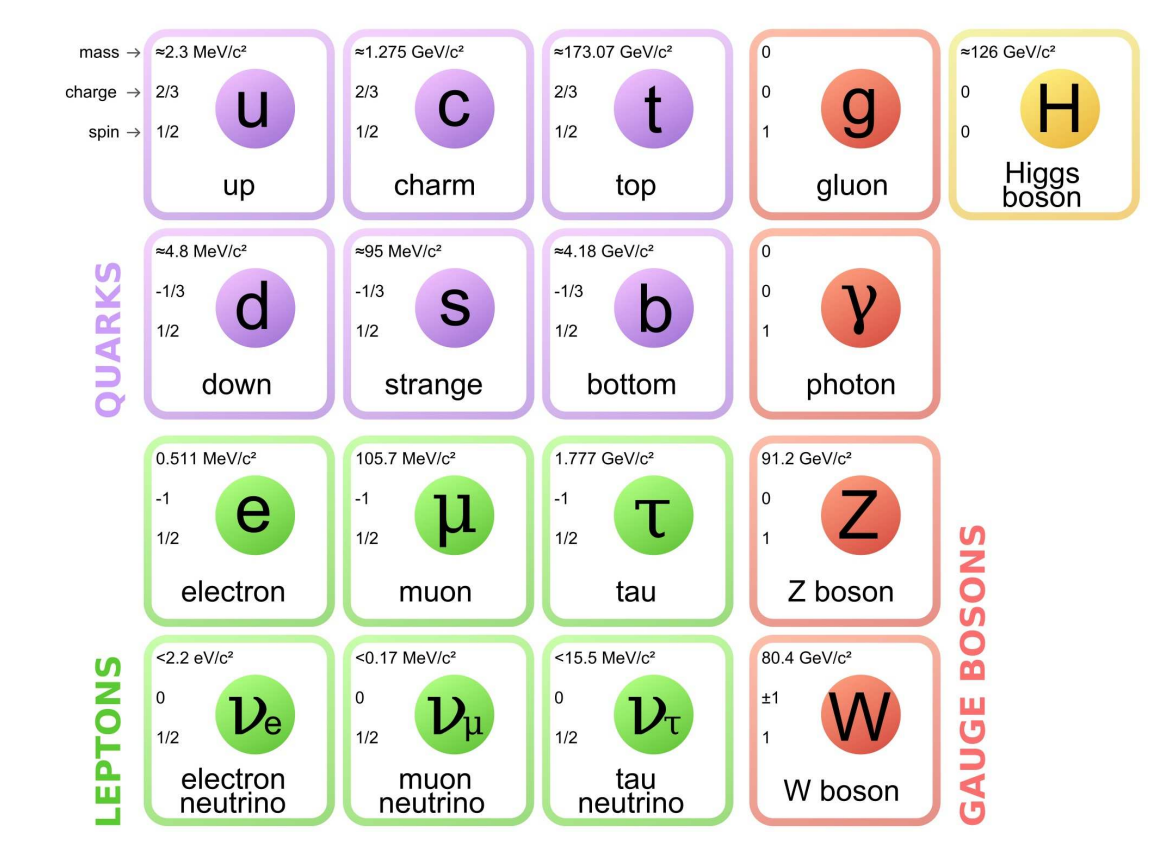
\includegraphics[scale=0.7]{sm.png}

The fermionic sector contains particle the particles that make up all known matter in the universe and is divided into the leptons and the quarks, both of this particles are divided into three generations, each generation being heavier than the one before. For the leptons we have electron and Its neutrino for the first generation, the second generation is. the $\mu$ and Its neutrino and the third one is the $\tao$ with Its neutrino. In the case of quearks we have the queark up and the quark down for the first generation, the second generation que have the quark charmd and the quark strange and for the third generation que have the quark top and the quark bottom. The bosons are the mediator particles called the gauge bosons already mentions, the photon, the gluon, the bosons $W\pm$ and the boson Z. There is also de Higgs bosson, which is the last gauge bossons and It's the responsible to give mass to the other SM particles  


One of the main sources to obtain elementary particles is particle accelerators, in this you acelerrate a particle into high energy and smash them with a target, with the proper  arrangements of magnets you can study the debris from the collision, for more heavy particles you need higher level of energy to the collision.

\section{Large Hadron Collider}

The Large Hadron Collider (LHC) is the biggest and powerful particle accelerator in the world, it consist in a 27 kilometers ring with superconducting magnets that boost the energy of the particles alongs the way. It uses proton beams from hydrogen tanks and there is four colliding points corresponding to different particle detectors, the ATLAS, the CMS, ALICE and LHCb. \cite{LHC}

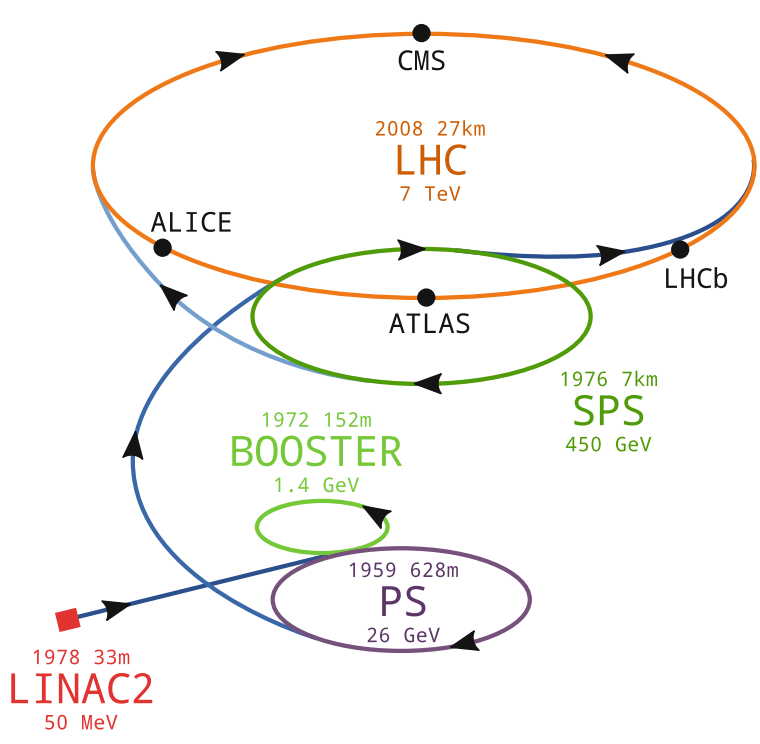
\includegraphics[scale=0.35]{LHC.png}



\section{Luminosity}
Luminosity is as key parameter in particle colliders

The luminosity is a quantity that measures the ability of the acelerator to produce the required number of interactions an is: 


$\frac{dR}{dt} = \mathcal{L} \cdot \sigma_{p} $ \cite{Lum} 


In which \cite{Lum}

In order to check the numbers of events the integrated luminosity is used and is defined as: 

$ L_{int} = \int L (t') dt' $



